\chapter{Babel.js}

\label{kap:babel} % id kapitoly pre prikaz ref

V tejto kapitole popisujem nástroj Babel.js.

Výsledná práca bude v angličtine, ale túto domácu úlohu píšem v slovenčine, lebo je to rýchlejšie. Preto som niekde použil anglický pojem, ak som nevedel slovenský ekvivalent.

Babel je nástroj slúžiaci na transpiláciu javascriptového kódu v najnovšej verzii ES2015 do formy, ktorá je podporovaná súčastnými internetovými prehliadačmi. Je napísaný v Javascripte. Vznikol v roku 2014 a v roku 2015 vyšiel vo verzii 6, ktorú sprevádzalo výrazné prepísanie a pluginy pre minulé verzie s ňou nie sú kompatibilné.

V nasledujúcom text popisujem jednotlivé fázy transpilácie a podsystémy, z ktorých sa skladá Babel.

\section{Fázy transpilácie}
Babel pracuje v troch fázach:
\begin{itemize}
\item lexikálna a syntaktická analýza zdrojového kódu,
\item transformácia abstraktného syntaktického stromu,
\item vygenerovanie finálneho zdrojového kódu z AST.
\end{itemize}

\subsection{Lexikálna a syntaktická analýza}
Počas lexikálnej analýzy sa zo zdrojového kódu tvorí zoznam tokenov (kategorizovaných reťazcov viac nedeliteľných znakov): napríklad kľúčové slová, reťazce, otváracie a zatváracie zátvorky. Tiež sa kontroluje, či je zdrojový kód v súlade s gramatikou.

Výstup lexikálnej analýzy programu \ref{listing:example} je možné vidieť v \ref{listing:lexical} (parametre loc a type sú objekty obsahujúce ďalšie údaje, ale kvôli prehľadnosti nie sú celé vypísané):

\begin{lstlisting}[caption=Ukážkový program,label=listing:example]
  function hello_world(name) {
	console.log("Hello World " + name);
  }
\end{lstlisting}


\begin{lstlisting}[caption=Výstup lexikálnej analýzy,label=listing:lexical]
  [
    {type: {label: "function", keyword: "function"},
      value: "function"},
    {type: {label: "name"}, value: "hello_world",},
    {type: {label: "("}},
    {type: {label: "name"}, value: "name"},
    {type: {label: ")"}},
    {type: {label: "{"}},
    {type: {label: "name"}, value: "console"},
    {type: {label: "."}},
    {type: {label: "name"}, value: "log"},
    {type: {label: "("}},
    {type: {label: "string"}, value: "Hello World "},
    {type: {label: "+/-"}, value: "+"},
    {type: {label: "name"}, value: "name"},
    {type: {label: ")"}},
    {type: {label: ";"}},
    {type: {label: "}"}},
    {type: {label: "eof"}
  ]
\end{lstlisting}

Následná lexikálna analýza na základe znalosti gramatiky jazyka vytvorí abstraktný syntaktický strom (AST) znázornený na grafe \ref{fig:ast}.

\begin{figure}[!htb]
  \centering
  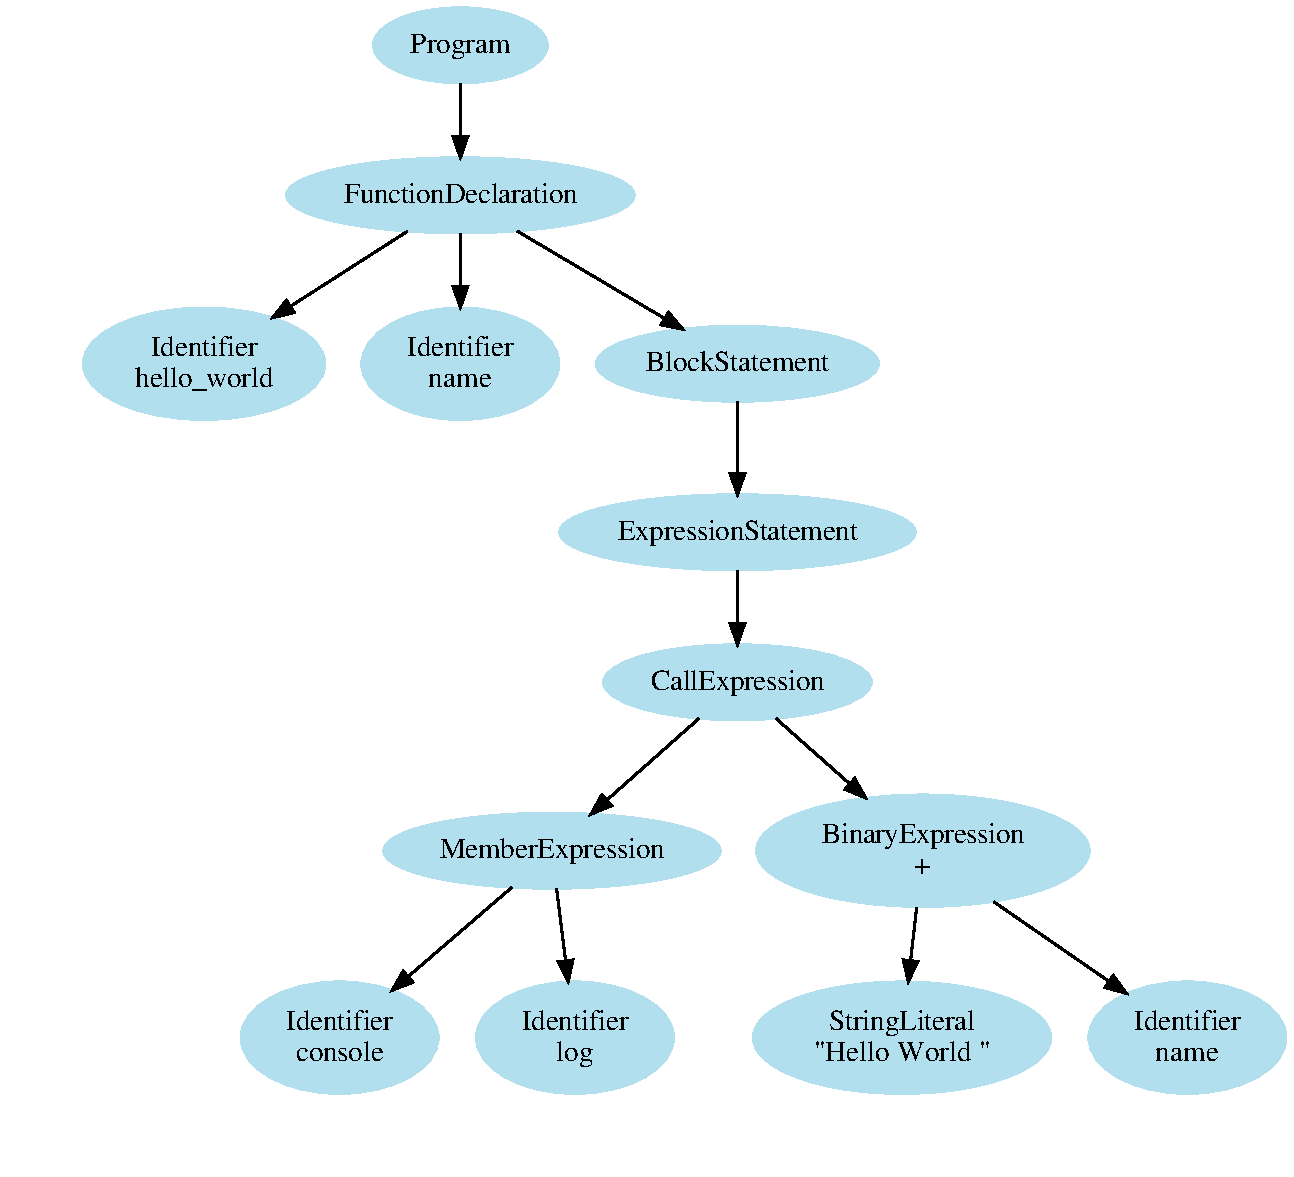
\includegraphics[scale=.7]{ast.eps}
  \caption{Abstraktný syntaktický strom.}
  \label{fig:ast}
\end{figure}

\subsection{Transformácia}
Transformácia AST je najvýznamnejšia fáza transpilácie, pri ktorej sa na strom aplikujú transformácie zadané tvorcom pluginu. Transformácia má formu návrhového vzoru visitor a udáva funkciu, ktorá sa vykoná pri navštívení vrcholu istého typu. Funkcia má prístup k parametrom daného vrchola a nadradeného vrchola a môže okrem iného:
\begin{itemize}
\item pridať nový vrchol pred alebo za navštívený vrchol,
\item nahradiť alebo odstrániť navštívený vrchol,
\item pridať premennú do ``scope'' (rozsah, v ktorom je platná),
\item premenovať existujúcu premennú,
\item spustiť nové prehľadávanie z navštíveného vrchola alebo niektorého zo synov.
\end{itemize}

\subsection{Generovanie}
Po vykonaní transformácií sa výsledný AST prehľadáva do hĺbky a jednotlivé vrcholy sa prepisujú do formy zdrojového kódu.

\section{Podsystémy}
Babel.js má modulárnu architektúru a skladá sa z viacerých balíčkov (npm packages), ktoré je možné použiť aj samostatne. Do veľkej miery kopírujú vyššie popísané fázy transpilácie.

\subsection{babylon}
Babylon je parser založený na pôvodnom parsere Acorn \cite{Acorn}, ktorý podporuje najnovší štandard ECMAScriptu a tiež neštandardizované rozšírenia syntaxe ako napríklad JSX \cite{JSX} alebo Flow \cite{Flow}. Jeho výstupom je AST.

\subsection{babel-traverse}
Babel-traverse je modul implementujúci prehľadávanie AST a udržiavanie jeho stavu, vrátene pridávania a odoberania vrcholov.

\subsection{babel-types}
Babel-types je modul zodpovedný za vytváranie a validáciu vrcholov a ich následný prepis do zdrojového kódu. Okrem štandardizovaných prvkov jazyka umožňuje tiež vytváranie nových.

\subsection{babel-generator}
Babel-generator je modul zodpovedný za prepis AST do výsledného zdrojového kódu spolu so ``source maps'' (technológia podporovaná všetkými modernými internetovými prehliadačmi definujúca mapovanie medzi pôvodným a transpilovaným zdrojovým kódom a umožňujúca tak jednoduchšie ladenie transpilovaného kódu).
